\documentclass[12pt,a4paper,oneside]{book} %%%%%%%%%%%%%%%%%%%%%%%%%%%%%%%%%%%%%%%%%%%%%%%%%

%%% preample %%%%%%%%%%%%%%%%%%%%%%%%%%%%%%%%%%%%%%%%%%%%%%%%%%%%%%%%%%%%%%%%%%


%%% packages %%%%%%%%%%%%%%%%%%%%%%%%%%%%%%%%%%%%%%%%%%%%%%%%%%%%%%%%%%%%%%%%%%

\usepackage[T1]{fontenc}        % euro quality fonts [T1] (togeth. w/ textcomp)
\usepackage{textcomp, amssymb}  % additional symbols (there are more packages)
\usepackage[utf8]{inputenc}   % umlaute in input file
\usepackage[english]{babel}     % newgerman: Worttrennung, Befehle f�r Umlaute
\usepackage{anysize}            % margin package sets tighter margins

\usepackage[a4paper,top=2cm,bottom=2cm,left=2cm,right=2cm]{geometry}

\usepackage{ifpdf}              % if pdflatex then ... else ...
%newer versions of latex don't need pdftex and dvips argument respectively
\ifpdf
  \usepackage{aeguill}          % PS converted CM fonts for better acro preview
  \usepackage[pdftex]{graphicx} % graphics packages
  \usepackage[pdftex]{color}    % color packages
  \usepackage[pdftex]{hyperref}
\else
  \usepackage[dvips]{graphicx}  % graphics packages
  \usepackage[dvips]{hyperref}
\fi

%%% style and finetuning %%%%%%%%%%%%%%%%%%%%%%%%%%%%%%%%%%%%%%%%%%%%%%%%%%%%%%

% pagestyle
\pagestyle{plain}               % headings, empty, plain

\hypersetup{colorlinks=false}   % don't print colored links on paper

% no indentation for paragraphs and space inbetween paragraphs  (euro standard)
\setlength{\parindent}{0pt}
\setlength{\parskip}{5pt plus 2pt minus 1pt}

\renewcommand{\baselinestretch}{1.05}

%%% hacks %%%%%%%%%%%%%%%%%%%%%%%%%%%%%%%%%%%%%%%%%%%%%%%%%%%%%%%%%%%%%%%%%%%%%

% hyperref must be (almost) last command of preample
% E.g. The \href{http://www.ctan.org}{CTAN} website.
% E.g. \author{First- Lastname $<$\href{mailto: email@domain}{email@domain}$>$}

\ifpdf
  \usepackage[pdftex]{hyperref}
\else
  \usepackage[dvips]{hyperref}
\fi
\hypersetup{colorlinks=false}   % don't print colors on paper
\usepackage{float}

\newcommand{\chapterimage}{nothing}

\newcommand{\newchapter}[2]{
    \renewcommand{\chapterimage}{#2}
    \chapter{#1}
}

\makeatletter
\renewcommand*{\@makechapterhead}[1]{
  \begin{figure}[H]
  \centering
  \thispagestyle{empty}
  \includegraphics[width=\textwidth,height=\textheight,keepaspectratio]{\chapterimage}
  \end{figure}
  \newpage
  {\Huge Chapter \thechapter: #1}
}
\makeatother


\begin{document}
%%% tile page %%%%%%%%%%%%%%%%%%%%%%%%%%%%%%%%%%%%%%%%%%%%%%%%%%%%%%%%%%%%%%%%%

\begin{titlepage}
\thispagestyle{empty}

\hrule
\begin{center}
{\bf\LARGE Hero History Apocrypha}

%\vspace{2cm}
%\begin{figure}[!htbp]
% \centering
% 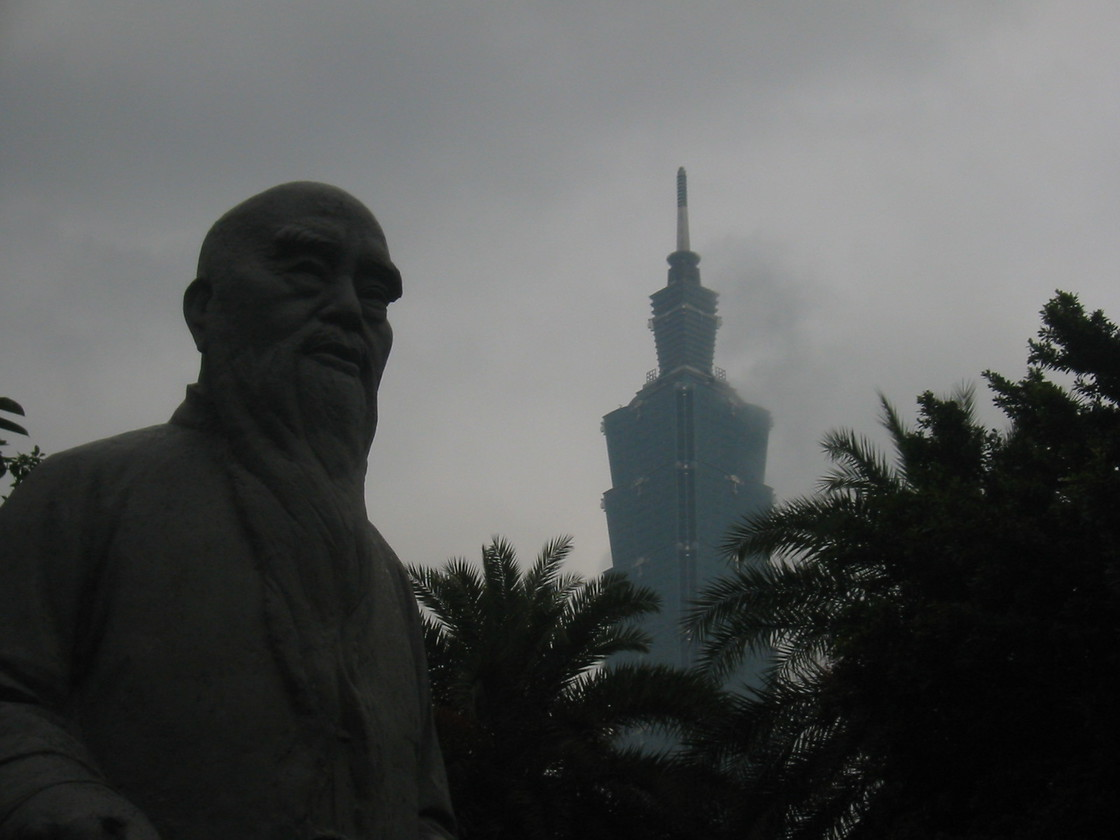
\includegraphics[width=1.0\textwidth]{images/cover_medium}
%\end{figure}

\end{center}
\end{titlepage}


\newpage %%%%%%%%%%%%%%%%%%%%%%%%%%%%%%%%%%%%%%%%%%%%%%%%%%%%%%%%%%%%%%%%%%%%%%

\setcounter{page}{1}\pagenumbering{roman}

\tableofcontents

\newpage

\setcounter{page}{1}\pagenumbering{arabic}

\part{Uesato Hinata is a Miko}
        
\newchapter{The Mikos}{uhimi-ch1-cover.jpg}

No human truly believes they will will one day die.

According to a literature-loving friend of mine, even Sigmund Freud, the founder of psychoanalysis, has said: ``As humans are incapable of accurately imagining their own death, they are thus incapable of truly believing their own death.''

Life is akin to walking on thin ice. Nobody knows when that ``death'' people don't even believe in will open its sinister jaws and swallow them.

Even the disaster that occurred in 2015 --- not that it was something as simple as disaster; I simply can't find a better expression --- was not something that anyone would believe would happen. But it did.

Vertexes. That was the name of the monsters that descended from the heavens, taking the lives of many people and destroying civilisation.

Amidst all that, special powers sprouted in some girls.

The power to stand against the Vertexes. The girls who manifested that power were called Heroes.

The power to receive oracles in order to guide the Heroes and the populace. The girls who manifested that power were called Mikos.

I, Aki Masuzu, was one of the Mikos.

``Cold! No way! I can't handle any more! I'm gonna die!''

2019, March. The winter cold still lingered strongly in those early spring days. I screamed those words out during our Mikos' daily waterfall purification ritual and dashed out of the waterfall.

``Aki-san, it hasn't even been two minutes yet...''  Those words, accompanied by a wry smile, came from Uesato Hinata, who was also purifying herself under the waterfall. That girl was also a Miko, and a year younger than me.

``Two minutes is enough time for instant noodles to cook! Besides, I've got a slender body with little body fat, so I'm weak against the cold. And we've got someone unforgivable here!''  I immediately started running towards that unforgivable ``someone''.

``Eh, Aki-san!? Where are you going?''  Uesato-chan followed right behind me.

I threw open the door to the Taisha public bath.

Behind that door someone was leisurely soaking in the bath while we Mikos were suffering under the cold waterfall.

``I'm going to take a bath too!'' I said as I jump into the bath.

``Wait, Aki-senpai! Please don't come in all of a sudden!''  With her face and hair wet from the splashing water, the girl - Hanamoto Yoshika - was glaring at me. I silently ignored her glare.

``Hee-hee, would it be okay if I joined as well? Purification by water really chills the body.''  Uesato-chan appeared from behind and came in as well.

``Mhm, it's fine. You come in too, Uesato-chan.''

``Why are you giving her permission, Aki-senpai? Please get out already, you're making the bath cramped.'' Hanamoto-chan glared at me.

``Ah, sorry. I'll leave if I'm bothering you,'' said Uesato-chan.

``No, it's fine. Uesato-san, soak into the bath and warm up. It would be bad if you caught a cold.''

``Wait a minute, Hanamoto-chan. Aren't you treating me and Uesato-chan way too differently?''

``Senpai, different people absolutely do not have the same worth. Doubly so for subjective worth in someone's eyes.''

``I have a feeling I'm being ridiculed by big words!''  I scooped up some water from the bath and splashed it at Yoshika. But that didn't manage to distort her cold expression even a little. Though since she didn't seriously try to chase me out of the bath, I didn't think Yoshika-chan actually hated me.

...Probably.

...Definitely.

...I hope so.

``Besides, it's your fault for being allowed not to stand under the waterfalls and getting to soak in the bath, Hanamoto-chan.''

Hanamoto-chan was a Miko, just like me and Uesato-chan, so she would also need to purify her body daily to serve the gods. She met my displeased look with a calm answer.  ``I can't enter water.''

That's right. She had aquaphobia. Even entering a warm knee-deep bath was a recent achievement for her; she couldn't possibly stand under a waterfall.

A while ago, when she first came under a waterfall, Hanamoto-chan threw up and lost consciousness. After that, she was allowed to purify herself in just bathwater.

``Warm bathwater is plenty enough for purifying the body. We're not monks in training, there's no need for asceticism. And besides, rituals get simplified all the time. When you enter a shrine, all you do is rinse your hands and mouth, right? That's a simplified purification ritual too, can't we do just that?''

``Oh... That's the kind of knowledge I'd expect from someone who's family owns a shrine. How about you let the higher-ups hear that reasoning of yours?''

Hanamoto-chan was born and raised at a shrine. Because of that, she knew a lot about religious stuff like gods and rituals.

``It's pointless. The things they and I believe in are different. They have their own beliefs,'' she said in a cold tone, shaking her head.

Uesato-chan folded her arms, listening to our talking. Stop it, your breasts are already too big for a middle-schooler and you're emphasizing them even more.  ``You're right... I'll talk to the Taisha priests. Doing waterfall purification in the cold months isn't good for the Mikos' wellbeing. I'll ask them to allow everyone to use bathing for purification just like Hanamoto-san.''

``Oh, that's good! The adults ought to listen if it's coming from you, Uesato-chan!''

When all was said and done, Uesato-chan had the strongest powers of all the Mikos. She was the most important Miko to the Taisha. They were bound to answer a request from her.

``If they insist that waterfall purification is necessary, I'll do it by myself. As long as that gets the other Mikos excused from it....''

``Eh? Uesato-chan, are you saying you're going to stand under the waterfalls all on your own?''

``Yes. If it's necessary.''

I let out a powerful sigh.  ``Then I'll do it with you too. I can't let a girl younger than me do something so harsh by herself.''

Uesato-chan calmly smiled and bowed her head.

Ah, jeez. I had wanted to get away from those waterfalls, but wasn't able to do it in the end. Her words would probably go through, too. Uesato-chan had managed to find a way for both me and the adults to save face and had found a compromise neither of us could refuse.

When Uesato-chan talked, this kind of stuff happened sometimes. She was on our side, but also on the Taisha's, so she tried to settle things as neutrally and conflict-free as possible.

Even if she had to pay the price before anybody else. It was really brave of Uesato-chan to be able to do that, but at the same time somewhat scary.

Now, three and a half years after 2015 when the Vertexes appeared and destroyed most of Japan, humans still survived in just a few places, or so we were told. The reason for that uncertain ``we were told'' is that we currently lived in Shikoku, but could not see the state of things outside it.

Shinju, said to be a congregation of the earthly gods, and a barrier that protects against Vertex attacks, had appeared in Shikoku. Thanks to them, humans could still live in this land. But because it was swarming with Vertexes outside the barrier, going outside it --- and thus, outside Shikoku --- was impossible. Which was why we didn't know how things are outside.

Right now, the organisation formed by the priesthood known as the Taisha [Grand Shrine] was in charge of the Vertex countermeasures.

The Taisha had gathered Heroes and Mikos under their control to stand against the Vertexes. The five Heroes in Shikoku all lived in their base, Marugame castle in the Kagawa prefecture. There were more Mikos than Heroes, and aside from Uesato-chan, who lived in the Marugame castle to keep watch over the Heroes, they all lived in Taisha facilities.

Among the Mikos, there were three central figures.

The first was Uesato Hinata. The best friend of Nogi Wakaba, a Hero, she guided her during the initial Vertex appearance. She had the strongest power of all the Mikos. She was in her second year of middle school and a year younger than me, but her breasts were big. They were huge.

The other one was Hanamoto Yoshika. She found Koori Chikage, a Hero, and she came from a shrine in the first place. She was a second-year, just like Uesato-chan. By the way, the kanji in her name read Yoshika, not Mika.

And then there was me, Aki Masuzu. I was a vivacious third-year who found the Heroes Doi Tamako and Iyojima Anzu! I was older than Uesato-chan and Hanamoto-chan, so I tried to act like their big sister, but I couldn't shake off the feeling Hanamoto-chan treats me really rudely. I knew I had to show her that I'm the older one here, but unfortunately I hadn't quite had the chance yet. Plus, since Uesato-chan was more proficient as a Miko and Hanamoto-chan was more knowledgeable, who knew if I'd ever get that chance.

By the way, aside from the four Heroes I already mentioned, there was another one. Takashima Yuuna was guided by a Miko called Karasuma Kumiko, but she was a lot older than the rest of us and it seemed she'd already lost her Miko powers. Right now, she served as a priestess at the Taisha.

Uesato-chan usually lived in the Marugame castle, but right now she was visiting the Taisha for a change.

``By the way, Uesato-chan, why are you at the Taisha today?'' I asked her after the bath while drying my hair.

``The Heroes will be going to explore what's outside of the barrier soon, so I was called in for a meeting to confirm the route.''

``...So they really are going to explore what's outside, huh.''

A little ago, the Heroes had fought and won a massive battle with the Vertexes, the Battle of the Marugame castle. For a while after that, the Vertex attacks on Shikoku stopped. So a plan to send the Heroes to scout outside of the barrier in this brief moment of peace for Shikoku was proposed. And it seemed they were going through with it.

Three and a half years had passed since the barrier protecting Shikoku formed. In that time, no exploration outside of Shikoku could be made because of the Vertex threat.

Until last summer, it was known that there were still people alive in Suwa in the Nagano prefecture, but it'd been half a year since that and nobody knew what was going on with Suwa now.

Hanamoto-chan, while changing, frowned anxiously.  ``Uesato-san, is it really okay for people to go outside the barrier? There's a rumour that outside of the barrier is brimming with toxins...''

``Yesterday, the Heroes went just slightly beyond the barrier to check the state of the earth, atmosphere and water. And not only is it not contaminated, the ecological situation is even better than before.''

Uesato-chan's words didn't make Hanamoto-chan's expression any brighter. It seemed her worries hadn't been dispelled.

With our morning purification ritual done, me and Hanamoto-chan go to the classroom. Uesato-chan goes to talk with the adults about the Heroes' expedition.

By the time we reached the classroom, most of the other Mikos were already there. It looked like we ended up late because we went to the bath after the waterfalls.

When it was time to start the lesson, a woman in her twenties wearing a white robe entered the classroom. It was Karasuma Kumiko, the former Miko. Aside from her work as a priestess, Karasuma-sensei was also the Mikos' teacher.

``Uh, alright, let's begin the lesson.''  Karasuma-sensei was almost listless. Apparently, she had been a graduate student before she entered the Taisha as a Miko, and quite a brilliant one at that, but she definitely didn't give off that expression.

The age of the Mikos was uneven, ranging from elementary school at the youngest to high school at the oldest. Because of that, it was impossible to teach everyone evenly. For that reason, most people studied on their own using textbooks and reference materials and asked Karasuma-sensei to explain parts they didn't understand. That was the teaching style.

All of the students were Mikos, but the studies weren't any different from what they had been learning in school before entering the Taisha. Even with our special powers, we still had the right to receive education. So we studied the same things they studied in normal schools.

While Karasuma-sensei was teaching the elementary schooler Mikos arithmetics, I shot a glance at Hanamoto-chan who was sitting next to me. She was looking at her notebook with a dubious expression. She wasn't a cheerful person in the first place, but it seemed she really was worried about the Heroes' expedition outside the barrier tomorrow.

I wrote ``Worried about the Heroes?'' on the edge of my notebook and showed it to Hanamoto-chan. Her mechanical pencil began to run across her own notebook.

``Even if there aren't any issues with the environment, we don't know how many Vertexes are out there. What if something happens to Koori-sama?''

``Hanamoto-chan, you worry too much. They'll be fine, the Heroes are crazy strong. That Nogi-chan is basically one foot in superhuman territory already.''

``Koori-sama is more delicate than the other Heroes. Aki-senpai, aren't you worried about Iyojima-sama and Doi-sama? You're friends, right?''

``Not really. Those girls have Hero powers, they'll manage.''

``You're cold.''

I was going to respond with something, but decided not to.

Now that I thought about it, how about Uesato-chan? Uesato-chan and the Hero Nogi-chan had been childhood friends since they were little; they were as close as family. I wonder if she was worried about Nogi-chan and the others going on an expedition outside the barrier.

The school lessons ended in the afternoon, and so did our time as ordinary middle school girls. Our time as Mikos of the Taisha began.

We learned norito prayers, were taught Shinto knowledge and practiced skills needed for rituals, like dancing and gagaku music.

And while we did that, the sun set. It became evening.

For dinner, we Mikos gathered in the cafeteria. Uesato-chan showed up in the cafeteria as well. Her meeting about the expedition must've ended.

The Mikos didn't have any dietary restrictions like the Buddhist ``meat is forbidden!'' That being said, our meals weren't exactly the same as they had been before we entered the Taisha. The dishes were mostly lightly flavoured, with vegetables and fish as the main parts, like something an adult who got a bad result on their health examination would eat. A bit lacking for us, since we were healthy and young.

Everyone said their thanks to the food and began to eat. No stiff ceremonies like offering prayers to the gods.

``Actually,'' said Yoshika-chan, ``Shinto has prayers to say before a meal. The adults in the Taisha must know that. I guess the words in that prayer don't quite fit in with the Shinju faith.''

Hanamoto-chan called the religion the Taisha taught the Shinju faith. I asked her once before how it was any different from Shinto. Hanamoto-chan explained it with a whole bunch of difficult terms like monotheism, polytheism, sect Shinto, ancient Shinto and so on. I responded with ``Uh-huh, got it.'' despite not having understood a thing. Hanamoto-chan must've also realised that I didn't understand anything.

Anyway, she said it should be called Shinju faith because it didn't worship all Japanese gods, but mostly Shinju-sama that appeared in Shikoku.

Some time ago, Hanamoto-chan was reprimanded by a Taisha priest for reciting a prayer her parents taught her because it was ``not appropriate''. It only makes sense that with that experience of hers, she'd find the ``Shinju faith'' different from shrine Shinto.

After dinner, the Mikos returned to the dorm. Like at a boarding school all of the Mikos lived at the dorm.

The Mikos were allocated one room for two people, and me and Hanamoto-chan were roommates. She was used to it now, but at the beginning Hanamoto-chan was really displeased about having to share a room with me. It wasn't because she hated me (or at least I liked to believe that!), but because she didn't like having other people around when sleeping.

In their rooms people reviewed their lessons and prepared for the upcoming ones, read manga or otherwise passed their time until it was lights out at 9 PM. The Mikos' day began early, so they went to bed early as well.

Mhm, very healthy.

This was how a Taisha Miko spent her days.

Well then, good night.

``...Yeah, like I could have a good night!''  I jumped out of the bed. I slept on the top bunk, and jumped up with such force I hit my head on the ceiling.

``What are you doing? Are you stupid? You're noisy.''  I heard Hanamoto-chan's cold voice as I was holding my head with tears in my eyes. It seemed that she, on the bottom bunk, had woken up as well.

``Going to bed at nine!? What are we, good kids? Elementary schoolers!?''

``What's wrong with being good kids? And there are elementary schooler Mikos, too.''

``Nuh uh! We're vivacious middle schoolers! We have to be a little unhealthy! Going to convenience stores and family restaurants in the middle of the night, going to clubs and narrowly avoiding getting chewed out! I want youthful stuff like that!''

``There aren't any convenience stores or family restaurants around, let alone clubs.''  Her reaction was calm and on point.

``I know that... But we have Uesato-chan here today, that's a rare occasion, so I want to stay up a bit longer. Alright, let's go to her room!''

``What, now...?''  Despite her displeased look, Hanamoto-chan still got up from her bed. It looked like she was coming with me. Hanamoto-chan, I liked that part of you.

And so, we went to Uesato-chan's room. Since she usually lived in the Marugame castle, she used the guest room whenever she came to the Taisha. Which was why she had a room to herself, without any roommates.

When we arrived, Uesato-chan guessed it all without our saying a word, smiled and let us in with a ``It's a secret from the priests.'' This girl was like the embodiment of tolerance. She may have been younger than me, but mentally she was definitely the older one.

``You came to visit me, but I don't have anything to offer... I don't even have games or anything to play...'' Uesato-chan said, as if apologising.

``Don't worry about it. It's Aki-senpai's fault for coming at this hour all of a sudden.''

``Heh heh heh. You two, better not underestimate your third-year senpai. I've got something we can play! Ta-da! Card mahjong!''

I raised up a thing that looks like a pack of playing cards, but much bigger.

Allow me to explain! Card mahjong is a convenient item that allows you to play mahjong as if it is a card game. You play mahjong using cards with mahjong tiles drawn on them. Since you don't get the feeling of slamming the tiles, it feels a bit lacking, but the appeal lies in the convenience provided by the ease of carrying the cards around.

``Ah, if it's mahjong, I'll pass,'' said Hanamoto-chan sharply.

``Me too...'' Uesato-chan awkwardly said the same.

``Eeh!? Let's play mahjong! I'm not saying to do it all night!''

``Aki-senpai, you've asked me over and over and I gave you this exact response every single time... I don't know mahjong rules at all. Besides, you're about the only middle schooler that can play mahjong, Aki-senpai, with your house being a mahjong parlor and all.''

``It's fine, I'll teach you! I'll teach you, okay!?''

Hanamoto-chan was cold. Absolute zero. An ice-cold woman.

Before I came to the Taisha, I often played mahjong with adults at my father's mahjong parlor. However, ever since I came to the Taisha, there hadn't been anybody I could play it with.

``Mahjong aside, we should probably arrange some drinks and sweets at least,'' Uesato-chan said with a wry smile.

``Then let's bring some.'' I grinned. ``The kitchen at the cafeteria ought to have some food and drinks. They might even have sweets.``

But the cafeteria was pretty far away from the room.

And we'd be busted if we got spotted by the patrolling Taisha personnel on the way there.

``I've lived here for over three years, I mostly know the staff's patrol routes and times at this point. We can do it!''

Mission start.

And the mission was pretty fun.

The three of us sneaked out of Uesato-chan's room. We couldn't use our smartphone flashes or flashlights, so I walked in the front in complete darkness, trying not to make a sound. When we reached a corner, I peeked out from behind the wall slightly, checking if anybody was in the corridor ahead. Since we couldn't use words, I gave Uesato-chan and Hanamoto-chan the OK hand sign, and we advanced further.

Finally, we arrived at the kitchen.

We took a bottle of barley tea from the fridge and borrowed some paper cups.

Uesato-chan found milk, eggs and bread, said ``It'd be sad with drinks only'' and whipped up french toast in a flash. ``For a quick bite instead of sweets,'' she said. It didn't even take her ten minutes to clean up the cooking utensils after herself.

What impressive household skills. Uesato-chan would definitely make a good wife. Though if you wanted to marry her, you'd have to get over the ridiculously high wall named Nogi Wakaba, the strongest in Shikoku.

By the way, we screwed up on the way back. We bumped into Karasuma-sensei walking down the hallway. It wasn't her time to patrol, so maybe she was on her way to the toilet or something. But Karasuma-sensei didn't say a thing. Our eyes definitely met, so she absolutely must have known it was us. But she yawned with boredom and walked away as if she hadn't seen a thing. Did she even understand she was a teacher?

We came back to the room and drank barley tea while munching on some french toast. And then we talked about various stuff.

Hanamoto-chan kept asking Uesato-chan: ``How is Koori-sama doing lately?'' Whether she was in good health, how her battle results were, what kind of games she had played recently, and so on...

``Hanamoto-chan, you really love Koori-chan, huh.''

``Of course I do. She's my Hero.''

Hanamoto-chan heard what games Koori-chan was playing from Uesato-chan and wrote everything down in her memo book. Apparently, she tried to play as many of those games as she could in order to have a conversation topic if she met Koori-chan.

But how often did she even meet with Koori-chan? The Mikos who lived on Taisha grounds and the Heroes who lived in the Marugame castle didn't intersect in their daily lives. I got to meet Tamako and Anzu-chan one, maybe two times a year.

Hanamoto-chan was the one who discovered Koori-chan when she manifested her Hero powers, so they must've met at least once then. But what about afterwards? We two had lived here at the Taisha for over three years, but I hadn't ever heard about Hanamoto-chan meeting up with Koori-chan.

Well, I guess it was none of my business.

``Oh yeah, Uesato-chan. About the Heroes' outside expedition, aren't you worried? About Nogi-chan and the others.''

``You're right. I trust them, but I can't help but be worried. Which is why I'm going with them.''

``Eh!? Uesato-chan, you're going too!? Isn't that dangerous!?''

Uesato-chan was a Miko, and unlike the Heroes, had no combat strength. She'd be helpless if the Vertexes attack.

``There's the possibility of an oracle from Shinju-sama, so at least one Miko has to accompany them. Which is why I offered to go with them. And besides... It'd be a lot harder for me to wait for their return.''

``...''

I couldn't say a thing.

A few days later, I heard that the Heroes and Uesato-chan had left on their expedition.

That day, after the lessons ended, I went to climb up a small mountain near the Taisha.

And the next day.

And the one after it.

You could see the sea from the top of that mountain. Beyond the sea, encircling Shikoku, stood the wall made out of what seemed to be plants. That wall was the boundary separating the inside of the barrier protecting Shikoku from the outside.

Beyond that wall it was swarming with the monsters named Vertexes. And amidst all that was Uesato-chan on her journey, with her fighting power no different from that of an ordinary person.

There's no way she wasn't scared, even if Nogi-chan was protecting her.

I closed my eyes.

Even three and a half years later, I could still vividly remember the first time I saw the Vertexes.

Eerie giant white monsters appeared all over Japan. Right in front of my eyes, too. Death opened its jaws at that moment. Death could've swallowed me at any moment.

After that day, I hadn't seen a Vertex up close. But if one did appear in front of me again, I'd probably freeze up in terror and start bawling. Even three and a half years ago, I was with two Heroes: Tamako and Anzu-chan. But I was still hopelessly scared of the Vertexes.

``Huff, huff... So that's where you were.''

I heard the voice and turned around to see Hanamoto-chan. She must have be tired from climbing up the mountain, because she was completely winded.

Hanamoto-chan caught her breath, adjusted the glasses that had slid off her nose and asked me, ``What are you doing all the way out here?''

``Uh, nothing special... I felt like looking at the sea.''

``You're worried about Doi-sama and Iyojima-sama, aren't you? Aki-senpai, you said that I worry too much, but aren't you the one who worries too much here? Aki-senpai, did you know? They call people like you `tsundere'.''

``T-That's not it! It's not like I'm worried...'' I tried to deny it, but stop.

``No, you're right. I am worried. Badly...''

``See, you should've admitted that from the start.''

``H-H-Hold on there! Why does it feel like I'm getting chewed out here!?''

``Because you put on pointless airs.''

I don't accept this...

I let out a sigh, sat down where I stood and looked up at the sky. I got my skirt dirty, but didn't pay any attention to that.  ``Listen. Hanamoto-chan, do you want to be at the Heroes' side like Uesato-chan?''

``Well... Who knows?'' she answered, looking up at the sky.

``You know, I have a little brother with the sky fear syndrome.''

A portion of humans who were attacked by the Vertexes developed PTSD. A large number of them were excessively afraid of the sky, from where the Vertexes appeared. Those with heavier symptoms were unable to walk under the sky, or even go outside at all. Some even went mad, beset by visual and auditory hallucinations. The condition was deemed to be possibly different from ordinary PTSD and was called uranophobia to differentiate. Its other name was sky fear syndrome.

``His condition is pretty heavy, so he's staying at a hospital all the time. Really, what I should be doing as his big sister is be with him. But I'm stuck inside the Taisha all the time, and I barely ever get to meet him...''

``You're a Taisha Miko, you can't do anything about that. Aki-senpai, could it be that you became a Miko so he could get preferential treatment?''

What a smart girl. It was just as Hanamoto-chan said. There were too many people with sky fear syndrome. Treating everyone was impossible. I had thought that if one of his family members was a Taisha Miko, he could get preferential treatment, and made the calculated decision to become one.

I don't want to imagine the worst, but I should probably try to meet him as often as I can. Because one day... We might not be able to meet again.

``You can't do anything,''  Hanamoto-chan said indifferently.  ``Aki-senpai, you can't do anything. Even if you're with your brother, you can't cure his uranophobia. Even if you're with the Heroes, your Miko powers aren't strong like Uesato-san's, so you can't do anything.''

``...Ahaha, what a horrible way to put it.''

``It's the truth. Aki-senpai, you should stay here at the Taisha and do what you can do. That would be the best for both your brother and the Heroes. Senpai, what you're doing now is the most rational course of action.''

``...''

She put it so horribly, but...

Maybe that was her way of cheering me up?

``...So what you're saying, Hanamoto-chan, is that I should stay in the Taisha, right? Do you want me to stay with you that much?''

``No.''

``Eh, but isn't that it? You said you want me to stay here, right? You must love me, Hanamoto-chan.''

``Keep that nonsense up and I'll punch you.''

``Cruel!''

But, well...

She was right: I was neither a doctor nor a psychologist; I couldn't cure my brother. My powers as a Miko weren't anywhere as high as Uesato-chan's, and more importantly, I didn't have her mental strength, so I wouldn't be very useful to the Heroes. If it were me, I would've probably been too scared of the Vertexes to follow the Heroes on their expedition outside.

``Overstepping one's bounds deals more damage than any cold can,'' Hanamoto-chan murmured.

``What does that mean?''

``It means that it's important to do your job and know what your duty is. Try to do more than that, and you'll only end up causing harm.''

Is that so?

Maybe it is.

I looked up at the sky again.

The clear blue sky was wide, deep and beautiful. You wouldn't think that the monsters that destroyed the human society came raining down from it. Before that happened, the sky had been a symbol of hope and luck for humanity. Now it was ominous and hated, but it was no less beautiful than before.

``Aah, why did we have to be born in such bad times?''

If I had been born somewhen normal, I would've been able to appreciate the beauty of this sky honestly.

I would've been able to sing praises to youth like a girl in middle school should.

And not just me, but Tamako and Anzu-chan, too...

``I'm glad I was born in these times,'' said Hanamoto-chan with no hesitation in her voice. It even sounded refreshing.  ``I was able to meet Koori-sama because I was born in these times, after all.''

The next day, the Heroes returned to Shikoku.

Both the Heroes and Uesato-chan were safe and sound; nobody was injured.

Hanamoto-chan and I were talking over lunch at the cafeteria.

``Uesato-chan and the others came back a lot sooner than I was expecting.''

``Yeah...'' said Hanamoto-chan with suspicion.

``The Heroes might move fast, but they couldn't have gone around all of Japan in this short of a time...''

We didn't know the exact route, but they were supposed to check the big cities like Osaka, Nagoya and Tokyo, as well as regions where there were still possible survivors: Suwa, Touhoku and even Hokkaido.

There was no way they managed to check so many places in just a mere three days.

``They turned back halfway through. Uesato received an oracle, apparently. That Shikoku is in imminent danger and they have to return quickly.''  That answer came from Karasuma-sensei, who happened to be eating nearby.

``Eh? But we haven't received an oracle like that...''

``Yeah. No Miko in the Taisha received it. But Uesato is a favourite of Shinju's, so it's not surprising that she'd be the only one to receive that oracle.''

That was Uesato-chan for you. But what could the imminent danger for Shikoku be?

``The Taisha is trying to figure out what that danger might be for the time being. And looking into the samples the Heroes brought back from their expedition. Well, I don't know how much good it'll do, but we'll try doing what we can.''  Having said that, Karasuma-sensei finished her meal, picked up her tray and stood up.

``The adults have it rough, too,'' I said to myself, looking at Karasuma-sensei's back.

The Mikos served Shinju-sama and received its oracles; that was our job. But aside from that, we were just children who couldn't do much else. All sorts of research and countermeasures --- it was all done by the Taisha.

``It's been over three years since I've entered the Taisha,'' said Hanamoto-chan with displeasure, ``But I still don't understand just what exactly this organisation is. If you ask me, few organisations in history have ever been as crooked as this one.''

\newpage
\thispagestyle{empty}
\includegraphics[width=\textwidth]{uhimi-ch1-1.jpg}




\end{document}


